
%%%%%%%%%%%%%%%%%%%%%%%%%%%%%%%%%%%%%%%%%
% Thin Sectioned Essay
% LaTeX Template
% Version 1.0 (3/8/13)
%
% This template has been downloaded from:
% http://www.LaTeXTemplates.com
%
% Original Author:
% Nicolas Diaz (nsdiaz@uc.cl) with extensive modifications by:
% Vel (vel@latextemplates.com)
%
% License:
% CC BY-NC-SA 3.0 (http://creativecommons.org/licenses/by-nc-sa/3.0/)
%
%%%%%%%%%%%%%%%%%%%%%%%%%%%%%%%%%%%%%%%%%

%----------------------------------------------------------------------------------------
%	PACKAGES AND OTHER DOCUMENT CONFIGURATIONS
%----------------------------------------------------------------------------------------

\documentclass[a4paper, 11pt]{article} % Font size (can be 10pt, 11pt or 12pt) and paper size (remove a4paper for US letter paper)

\usepackage[protrusion=true,expansion=true]{microtype} % Better typography
\usepackage{graphicx} % Required for including pictures
\usepackage{wrapfig} % Allows in-line images
\usepackage{listings}             % Include the listings-package
\usepackage[utf8]{inputenc}
\usepackage{mathpazo} % Use the Palatino font
\usepackage[T1]{fontenc} % Required for accented characters
\linespread{1.05} % Change line spacing here, Palatino benefits from a slight increase by default
\usepackage{color}
\usepackage{graphicx}
\makeatletter
\renewcommand\@biblabel[1]{\textbf{#1.}} % Change the square brackets for each bibliography item from '[1]' to '1.'
\renewcommand{\@listI}{\itemsep=0pt} % Reduce the space between items in the itemize and enumerate environments and the bibliography

\lstset{numbers=left, frame=single,}

\definecolor{codegreen}{rgb}{0,0.6,0}
\definecolor{codegray}{rgb}{0.5,0.5,0.5}
\definecolor{codepurple}{rgb}{0.58,0,0.82}
\definecolor{backcolour}{rgb}{0.95,0.95,0.92}
 
\lstdefinestyle{mystyle}{
    backgroundcolor=\color{backcolour},   
    commentstyle=\color{codegreen},
    keywordstyle=\color{magenta},
    numberstyle=\tiny\color{codegray},
    stringstyle=\color{codepurple},
    basicstyle=\footnotesize,
    breakatwhitespace=false,         
    breaklines=true,                 
    captionpos=b,                    
    keepspaces=true,                 
    numbers=left,                    
    numbersep=5pt,                  
    showspaces=false,                
    showstringspaces=false,
    showtabs=false,                  
    tabsize=2
}

\renewcommand{\maketitle}{ % Customize the title - do not edit title and author name here, see the TITLE block below
\begin{flushright} % Right align
{\LARGE\@title} % Increase the font size of the title

\vspace{50pt} % Some vertical space between the title and author name

{\large\@author} % Author name
\\\@date % Date

\vspace{40pt} % Some vertical space between the author block and abstract
\end{flushright}
}

%----------------------------------------------------------------------------------------
%	TITLE
%----------------------------------------------------------------------------------------

\title{\textbf{Przegląd wybranych generatorów liczb pseudolosowych}\\ % Title
i analiza ich widma spektralnego.} % Subtitle

\author{\textsc{Mateusz Sołtysik, Andrzej Kwak, Wiktor Dyngosz} % Author
\\{Politechnika Wrocławska, \textit{Wydział Podstawowych Problemów Techniki}}} % Institution

\date{Czerwiec, 2014} % Date

%----------------------------------------------------------------------------------------

\begin{document}

\maketitle % Print the title section
\pagebreak

%----------------------------------------------------------------------------------------
%	ABSTRACT AND KEYWORDS
%----------------------------------------------------------------------------------------

%\renewcommand{\abstractname}{Summary} % Uncomment to change the name of the abstract to something else

\section*{Wstęp}
Pseudo-Random Number Generator (PRNG) – program lub podprogram, który na podstawie niewielkiej ilości informacji (ziarno, ang. seed) generuje deterministyczny, potencjalnie nieskończony, ciąg liczb.
\\Przykłady zastosowań generatorów liczb pseudolosowych:
\begin{enumerate}
\item Kryptografia
\item Całkowanie numeryczne (metoda Monte-Carlo)
\item Symulacja systemów masowej obsługi
\item Automaty do gier losowych
\end{enumerate}
Generatory liczb pseudolosowych nie generują ciągów prawdziwie loso-wych - generator inicjowany ziarnem, które może przyjąć $k$ różnych wartości, jest w stanie wyprodukować co najwyżej $k$ różnych ciągów liczb. Ponieważ rozmiar zmiennych reprezentujących wewnętrzny stan generatora jest ograniczony i może on znajdować się tylko w ograniczonej liczbie stanów, po pewnym czasie generator dokona pełnego cyklu i zacznie generować te same wartości.
\\Pożądane cechy generatorów:
\begin{enumerate}
\item Trudne do ustalenia ziarno, choć znany jest ciąg wygenerowanych bitów
\item Trudne do ustalenia kolejno generowane bity, choć znany jest ciąg bitów dotychczas wygenerowanych
\end{enumerate}
Teoretyczny limit długości cyklu wyrażony jest przez $2^n$, gdzie $n$ to liczba bitów przeznaczonych na przechowywanie stanu wewnętrznego. W praktyce, większość generatorów ma znacznie krótsze okresy.
W tej pracy przedstawiamy opis, zasadę działania oraz analizę widma spektralnego wymienionych algorytmów:
\begin{enumerate}
\item Blum Blum Shub
\item Liniowy Generator Kongruentny (LCG)
\item Mersenne twister
\item Generator Parka-Millera
\item Xorshift
\item Wichmann and Hill
\item Linear feedback shift register
\item RC4
\item Multiply-With-Carry
\end{enumerate}
\pagebreak
%----------------------------------------------------------------------------------------
\section{Opis i analiza algorytmów PRNG}
\subsection*{Informacje wstępne}
Każdy - opisany w tej pracy - algorytm, powinien być inicjowany tzw. seedem. Przypomnijmy, że dany algorytm z ustalonymi parametrami i znaną wartością seed, generuje te same ciągi! Aby zapobiec przekłamaniom w tym zakresie postanowiliśmy, że nasza implementacja będzie korzystała z funkcji $getSeed()$, która przy procesie generacji ziarna wykorzystuje niedeterministyczne źródło bitów ($/dev/urandom$). \begin{lstlisting}[style=mystyle, language=java, frame=single, caption = Przykładowa funkcja generująca seed.]
public static long getSeed() {
      SecureRandom random = new SecureRandom();
      byte seed[] = random.generateSeed(20);
      return Longs.fromByteArray(seed);
}
\end{lstlisting}
\subsection*{Testy spektralne}
Analiza spektralna algorytmu służącego do generowania liczb pseudolosowych polega na wygenerowaniu liczby próbek $p$ par uporządkowanych kolejnych liczb $(x_{i}, x_{i+1})$ dla $i \in 0,1,2,\dots,p-1$. W ramach tej pracy została zaimplementowana lista algorytmów oraz stworzony program GUI, który umożliwia przeprowadzanie owych testów. \\
Testy dla każdego algorytmu nie powinny przekraczać wartości $10^{9}$, ponieważ zakres 32-bitowej liczby jest równy $\frac{32\log(2)}{\log(10)} \approx 9$.

%----------------------------------------------------------------------------------------
\subsection{Blum Blum Shub}
Algorytm \textit{Blum Blum Shub} został zaproponowany przez Lenore Blum, Manuela Blum'a oraz Michaela Shub'a wiosną, 1986. roku, w pracy: "A Simple Unpredictable Pseudo-Random Number Generator"\footnote{http://epubs.siam.org/doi/abs/10.1137/0215025}. Generator ten jest postaci:
\[ x_{n+1} = (x_{n})^2 \bmod N \]
gdzie $x_{n+1}$ to kolejny stan generatora, $N$ to iloczyn dwóch dużych liczb pierwszych $p$ i $q$ takich, że:
\begin{enumerate}
\item dają w dzieleniu przez 4 resztę 3 ($p\equiv q \equiv 3 \bmod 4$),
\item mają możliwie mały $NWD(\phi(p-1), \phi(q-1))$, co zapewnia długi cykl.
\end{enumerate}
Wynikiem generatora jest kilka ostatnich bitów $x_{n}$.
\begin{lstlisting}[style=mystyle, language=java, frame=single, caption = Generowanie następnej liczby pseudolosowej przez BBS]
private static final int p = 11;
private static final int q = 19;

public static long getRandomNumber() {
    seed = (seed * seed) % (p * q);
    return Math.abs(seed);
}
\end{lstlisting}
Generator ten jest nie jest najszybszy, jednakże jest bardzo bezpieczny. Przy odpowiednich założeniach, odróżnienie jego wyników od szumu jest równie trudne co faktoryzacja $N$.\\
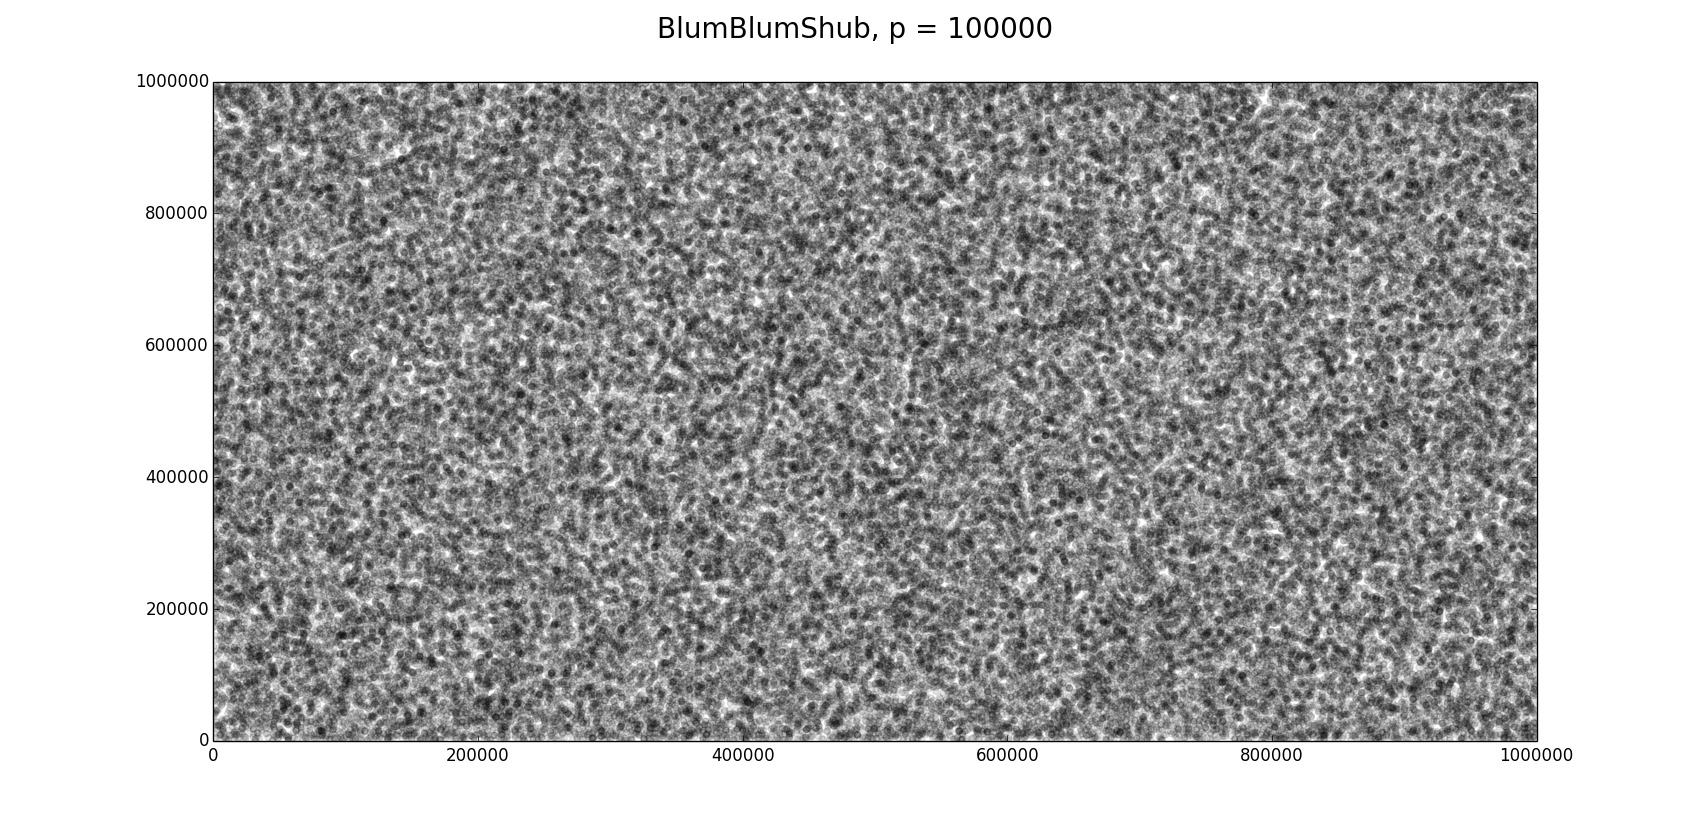
\includegraphics[width=\linewidth]{img/bbs-1.png}
%----------------------------------------------------------------------------------------
\subsection{Liniowy Generator Kongruentny (LCG)}
Liniowe Generatory Kongruentne to najbardziej rozpowszechnione w praktyce algorytmy PRNG. Wyróżniamy dwa rodzaje tych generatorów:
\begin{enumerate}
\item Addytywne\\
W postaci: $x_{i+1}=(a*x_{i}+c) \bmod m$
\item Multiplikatywne\\
W postaci: $x_{i+1} = (a * x_{i}) \bmod m$, gdzie:
\end{enumerate}
$x_{i+1}$ to kolejna liczba pseudolosowa,\\
$m, 0 < m$ - zakres generowanej liczby\\
$a, 0 < a < m$ - współczynnik mnożenia\\
$c, 0 \le c < m$ - współczynnik inkrementacji\\
Dla pewnych kombinacji parametrów generowany ciąg jest prawie losowy, dla innych
bardzo szybko staje się okresowy. Cechą tych generatorów jest również fakt, iż jeśli kolejna wygenerowana liczba powtarza się w ciągu liczb już wygenerowanych, to wpadamy w cykl: $x_{1}, x_{2},\dots,x_{1},x_{2}$. Mimo bardzo prostej budowy i zasady działania, powstało wiele prac i analiz matematycznych, które mówią nam o najlepszym doborze parametrów $m, a, c$. Najlepszym, to znaczy takim w którym cykl będzie jak najdłuższy. Przykładowe zalecenia: \\
\begin{enumerate}
\item Parametr $m$ powinien być duży, najlepiej wielokrotnością $2$ (najczęsciej spotyka się generatory LCG, w których $m = 2^{32}$ lub (w nowszych) $m = 2^{64}$)
\item Parametr $a$ powinien być o jeden rząd mniejszy niż $m$.
\item Dobrą wartością dla $a$ jest liczba postaci $t21$, gdzie $t$ - liczba parzysta.
\end{enumerate}

\begin{lstlisting}[style=mystyle, language=java, frame=single, caption = Generowanie następnej liczby pseudolosowej przez LCG]
private final static long a = 6364136223846793005L;
private final static long b = 1442695040888963407L;
private final static long m = (long) Math.pow(2, 64);

public static long getRandomNumber() {
    seed = (a * seed + b) % m;
    return seed;
}
\end{lstlisting}
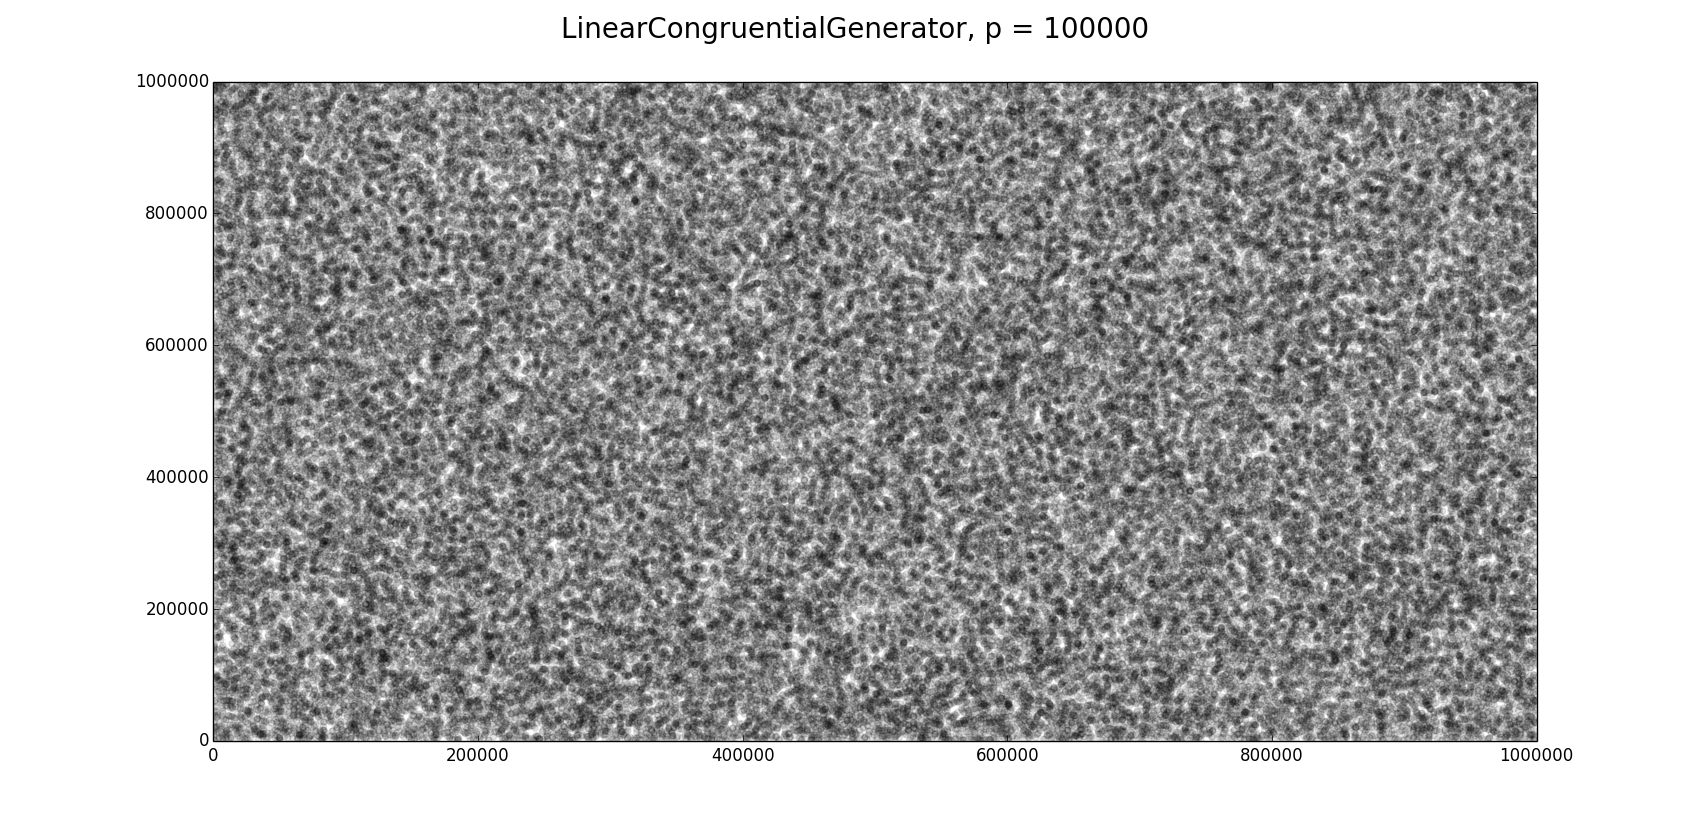
\includegraphics[width=\linewidth]{img/lcg-2.png}
%----------------------------------------------------------------------------------------
\subsection{Mersenne twister}

\textit{Mersenne twister} został opracowany przez Makoto Matsumoto i Takuji Nishimura w 1997 roku\footnote{http://doi.acm.org/10.1145/272991.272995}. Generator ten dostarcza wysokiej jakości liczby pseudolosowe oraz jest bardo szybki. Nazwa pochodzi od tego, że na dlugość okresu została wybrana pierwsza liczba Mersenne'a. Algorytm, mimo swoich zalet, nie nadaje się do zastosowań kryptograficznych. Stosunkowo obserwacja niewielkiej liczby iteracji (624) pozwala przewidzieć wszystkie kolejne. Kolejną kwestią jest dlugi czas inicjalizacji algorytmu - w porównaniu do generatora Fibonacciego lub liniowego generatora kongruencyjnego. 
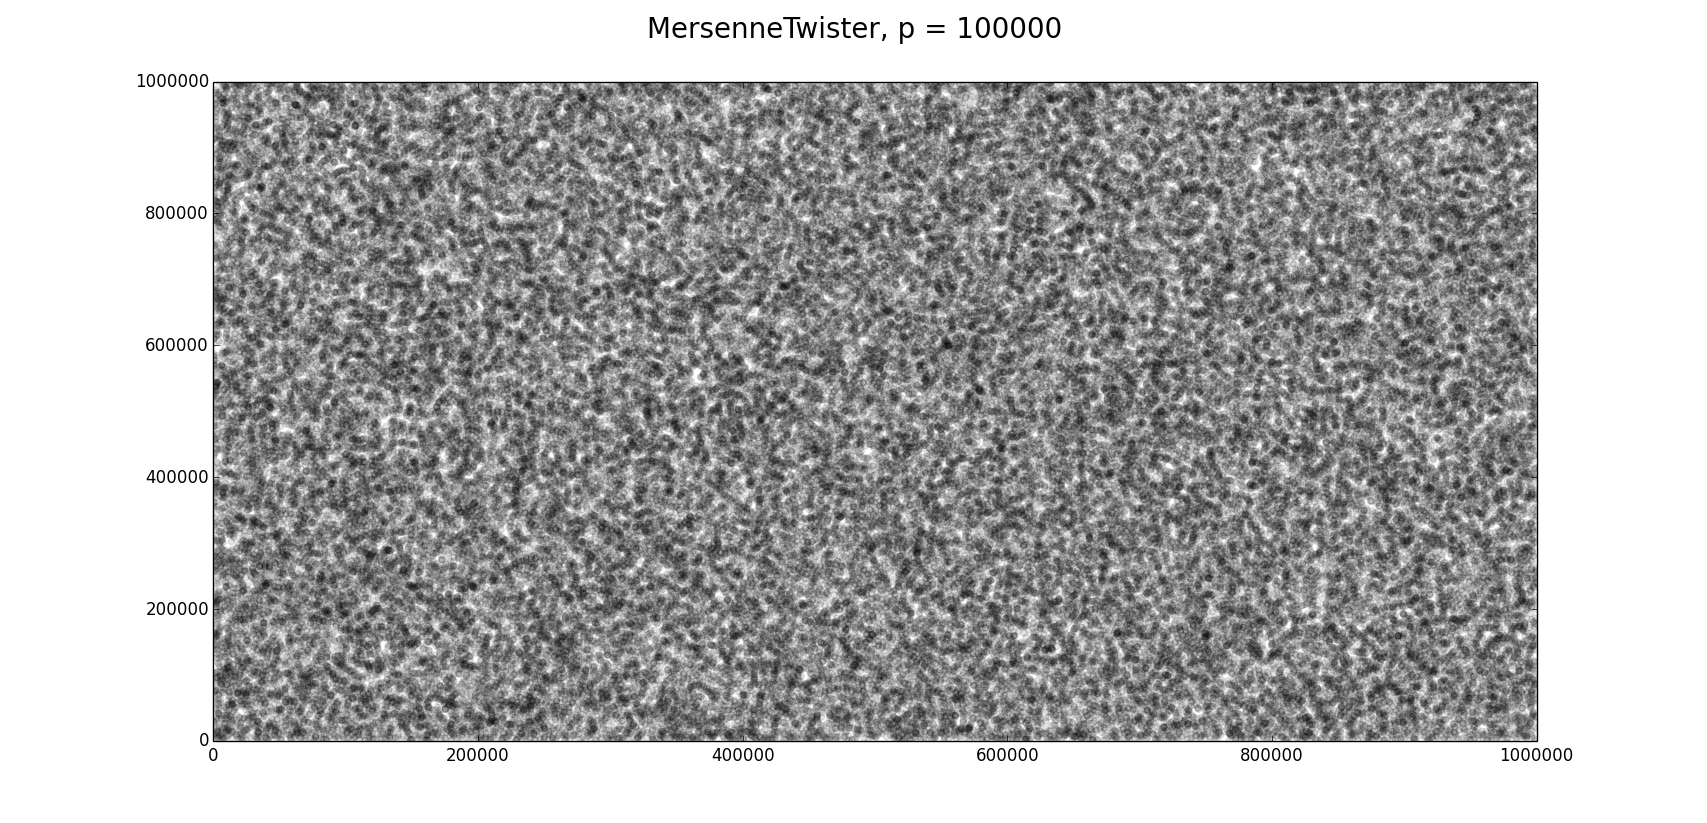
\includegraphics[width=\linewidth]{img/mt-1.png}

%----------------------------------------------------------------------------------------
\subsection{Generator Park–Miller}
Generator jest odmianą multiplikatywnego liniowego generatora kongruencyjnego, który określamy wzorem:
\[ x_{n+1} = (a * x_{n}) \bmod M \]
gdzie, $x_{n+1}$ to następna liczba pseudolosowa, $a$ - współczynnik generujący kolejną liczbę, $M$ - współczynnik określający zakres generowanych liczb (od $0$ do $M-1$).
\begin{lstlisting}[style=mystyle, language=java, frame=single, caption = Generowanie następnej liczby pseudolosowej przez algorytm Parka-Millera.]
private static final long max = ((long) 2 << 30) - 1;
private static final long a = 16807;

public static long getRandomNumber() {
    seed = (a * seed) % max;
    return seed;
}
\end{lstlisting}
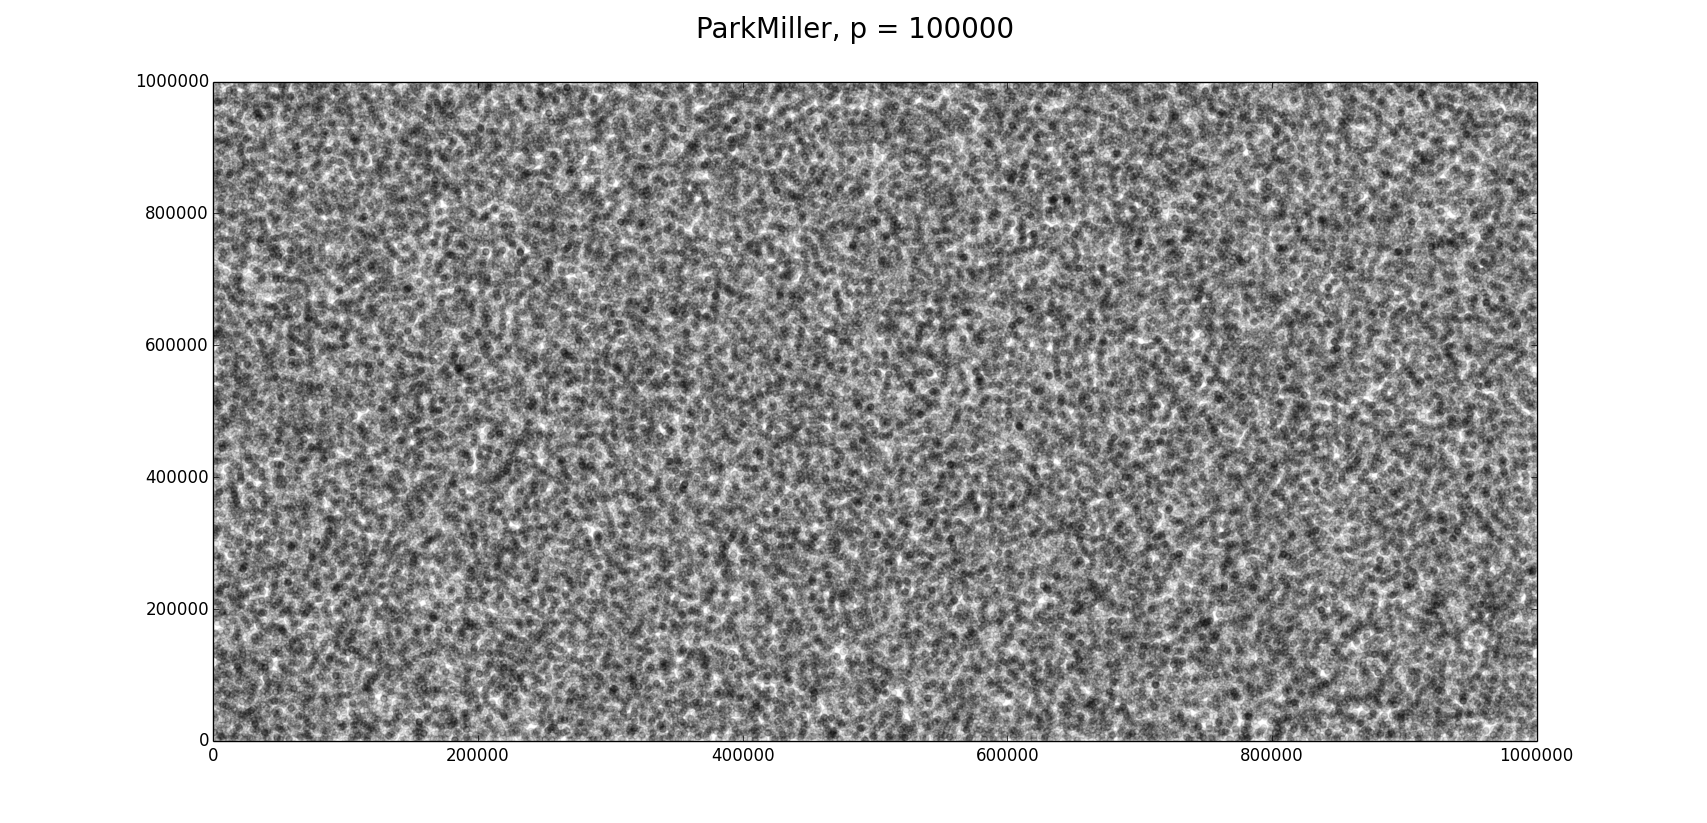
\includegraphics[width=\linewidth]{img/pm-1.png}
%----------------------------------------------------------------------------------------
\subsection{Xorshift}
Algorytm został zaproponowany przez George Marsaglia\footnote{http://www.jstatsoft.org/v08/i14/paper} w 2003 roku. Liczba $x_{n+1}$ jest generowana poprzez wielokrotną różnicę symetryczną liczb $x_{n}$ i przesuniętej bitowo $x_{n}$. Wykorzystanie funkcji $XOR$ sprawia, że ten algorytm jest niezwykle szybki na współczesnych komputerach.
\\
Algorytm ten jest szybki ale nie niezawodny i z pewnością nie nadaje się do zastosowań kryptograficznych. Jednak, połączenie go z nieliniowym generatorem - jak pierwotnie sugerował autor - prowadzi do jednego z najszybszych generatorów, spełniających silne wymogi testów statystycznych.

\begin{lstlisting}[style=mystyle, language=java, frame=single, caption = Generowanie następnej liczby pseudolosowej przez Xorshift]
public static long getRandomNumber() {
    seed ^= seed >> 12;
    seed ^= seed << 25;
    seed ^= seed >> 27;
    seed = (seed * 2685821657736338717L) % max;
    return Math.abs(seed);
}
\end{lstlisting}
Silnik przeglądarki internetowej Webkit korzysta z tego algorytmu przy wywoływaniu $Math.random()$ w języku JavaScript.\\
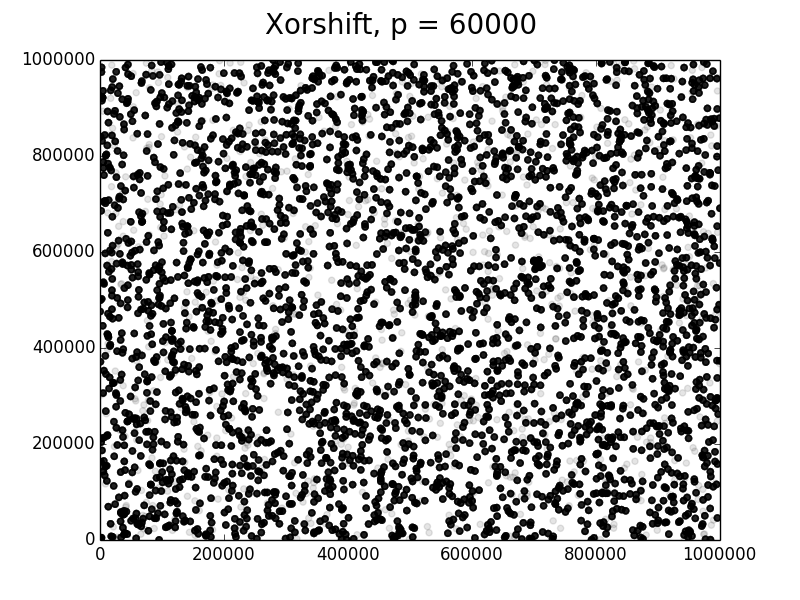
\includegraphics[width=\linewidth]{img/xorshift-1.png}
%---------------------------------------------------------------------------------------- %
\subsection{Wichmann and Hill}
Algorytm został zaproponowany przez autorów w 1982 roku. Jego przybliżony okres wynosi $2^{43}$ z tego powodu generator stał się bardzo popularny. Algorytm wykorzystuje kombinacje trzech liniowych generatów kogruentnych (LCG). Na początku inicjalizowane są trzy wartości $I_x$, $I_y$, $ I_z$ które przyjmuja wartości od 1 do 30,000. Następnie wykonywane są następujące operacje: 
$$I_x := 171 \times (I_x  \bmod  177) - 2 \times (I_x : 177) $$
$$I_y := 172 \times (I_y  \bmod 176) - 35 \times (I_y : 176) $$
$$ I_z := 170 \times (I_z \bmod  178) - 63 \times (I_z : 178)$$
\textbf{if}$I_x < 0$ \textbf{then}
\newline \indent	$I_x := I_x + 30269;$

\noindent \textbf{if}$I_y < 0$ \textbf{then}
\newline \indent	$I_y := I_y + 30307;$

\noindent \textbf{if}$I_z < 0$ \textbf{then}
\newline \indent	$I_z := I_z + 30323;$
\noindent \newline $W := I_x/30269.0 + I_y/30307.0 + I_z/30323.0$
\newline W pracy przy implementacji algorytmu skorzystano z faktu, że WH RNG może być zapisany jako prosty generator kongruentny za pomocą wzoru: 
$$X_{n+1} = 16555425264690 \times X_n\ mod\ 27817185604309 $$
znanego także jako rekursja Zeisela.

\begin{lstlisting}[style=mystyle, language=java, frame=single, caption = Generowanie następnej liczby pseudolosowej przez algorytm Wichmanna-Hilla na podstawie rekursji Zeisela.]
    public long getRandomNumber() {
        seed = (16555425264690L * seed) % 27817185604309L;
        return Math.abs(seed);
    }
\end{lstlisting}
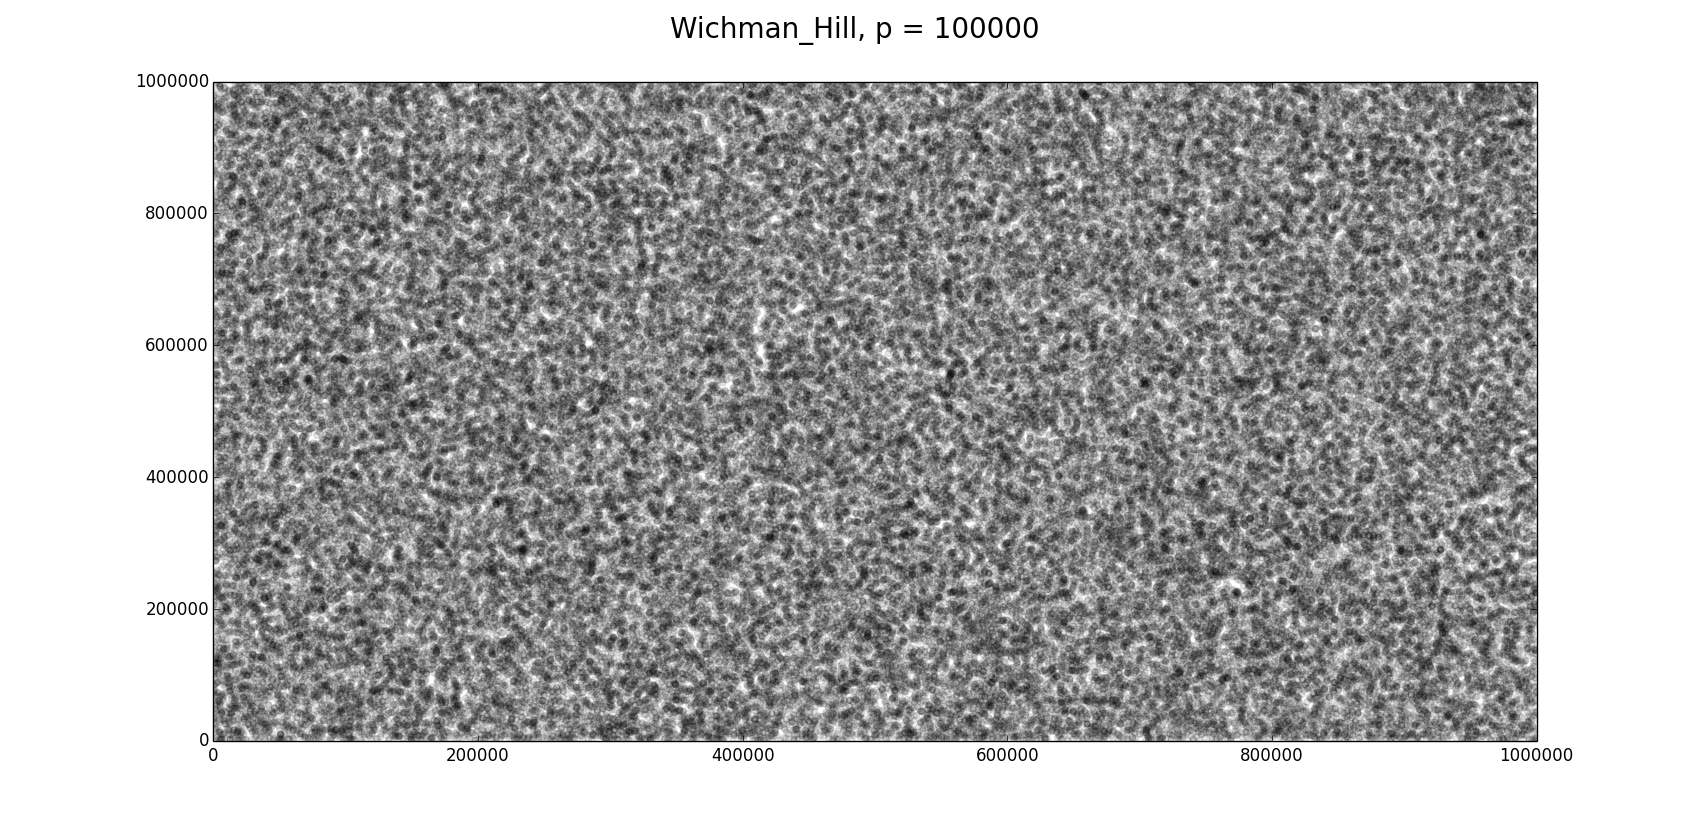
\includegraphics[width=\linewidth]{img/wh-1.png}

%----------------------------------------------------------------------------------------------------------------- %
\subsection{Linear feedback shift register}
\textit{Linear feedback shift register} albo inaczej Rejestr przesuwający z liniowym sprzężeniem zwrotnym to generator, którego bit wejściowy jest funkcją jego poprzedniego stanu. Wartość początkowa rejestru jest jego ziarnem. Następnie ustalone funkcje konkretnych komórek rejestru XORują wynik bitu wychodzącego.
\begin{lstlisting}[style=mystyle, language=java, frame=single, caption = generowanie liczby za pomocą LFSR i przesuwanie komórek.] 
        // wygeneruj liczbe losowa
        int next = 0;
        for (int i = 0; i < M; i++) {
            next |= (bits[i] ? 1 : 0) << i;
        }

        // przesun na zero jesli liczba ujemna
        if (next < 0) next++;

        // wylicz ostatni rejestr ze stanow okreslonych rejestrow
        bits[M] = false;
        for (int TAP : TAPS) {
            bits[M] ^= bits[M - TAP];
        }

        // przesuwanie rejestrow
        System.arraycopy(bits, 1, bits, 0, M);

        return Math.abs(next);
    
\end{lstlisting}
Jak widzimy na powyższym listingu liczba generowana jest za pomocą obecnych stanów tablicy. Po wylosowaniu wyrzucany jest ostatni bit i jest xorowany z określonymi przez nas komórkami. Następnie tablica jest przesuwana o 1. \newline
Każdy LFSR jest związany z określonym wielomianem z pierścienia wielomianów R[t], gdzie R jest ciałem skończonym $Z_2$.
Okres rejestru jest ograniczony przez stopień stowarzyszonego z nim wielomianu i wynosi maksymalnie $2^d - 1$, gdzie d jest stopniem wielomianu (ciało ${Z}_2$ ma charakterystykę równą 2). Okres danego LFSR jest maksymalny jeżeli stowarzyszony z nim wielomian jest wielomianem pierwotnym. Rejestr taki, nazywamy rejestrem maksymalnej długości.
\newline Zaletą LFSR jest niesamowita szybkość wynikająca z operacji logicznych przez co znalazł on zastosowanie w szyfrach strumieniowych.\\
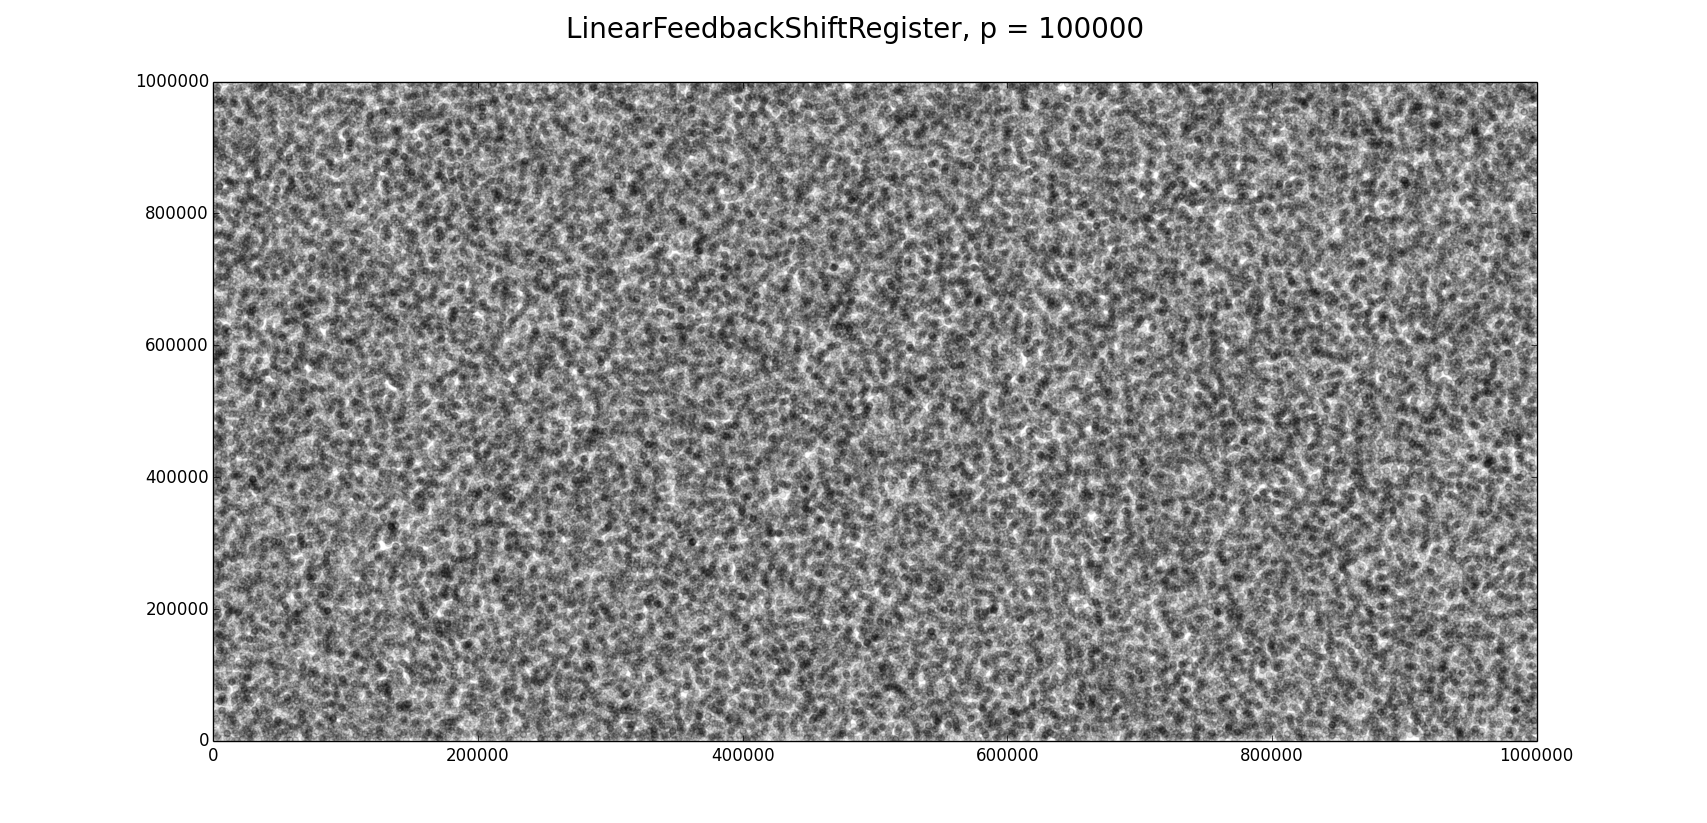
\includegraphics[width=\linewidth]{img/lfsr-1.png}

%---------------------------------------------------------------------------------------- %
\subsection{RC4}
\textit{RC4} to szyfr strumieniowy, wymyślony przez Rona Rivesta w 1987 roku. Algorytm opiera się na 256 elementowej tablicy i dwóch wskaźnikach. Początkowo tworzona jest permutacja identycznościowa. Następnie w 256 iteracjach tablica jest przetwarzana i mieszana z bajtami klucza.
\begin{lstlisting}[style=mystyle, language=java, frame=single, caption = Inicjalizowanie RC4.]
        String key = Long.toHexString(seed);
        int j = 0;
        for(int i = 0; i < 256; i++){
            j = (j + list.get(i) + (int) key.charAt(i%key.length())) % 256;
            int tmp = list.get(i);
            list.set(i, list.get(j));
            list.set(j, tmp);
\end{lstlisting}
Następnie do generowania kolejnych bitów liczby, ponownie tablica jest przetwarzana.\\ Każdy element tablicy jest permutowany conajmniej raz podczas 256 iteracji.
\begin{lstlisting}[style=mystyle, language=java, frame=single, caption = Generowanie losowego bajtu liczby za pomocą RC4.]
    private String prga(){
        int i,j;
        i = j = 0;
        for(int k = 0; k < 256; k++) {
        	i = (i+1) % 256;
        	j = j + list.get(i) % 256;

        	int tmp = list.get(i);
        	list.set(i, list.get(j));
        	list.set(j, tmp);
        }
        int t = list.get((i+j)%256);
        return Integer.toHexString(list.get(t));
    }
\end{lstlisting}
Dużą zaletą tego szyfru jest jego szybkość. Generator znacznie wydajniej generuje bity od liniowych generatorów. Algorytm wykorzystywany jest w systemach OpenBSD.\\
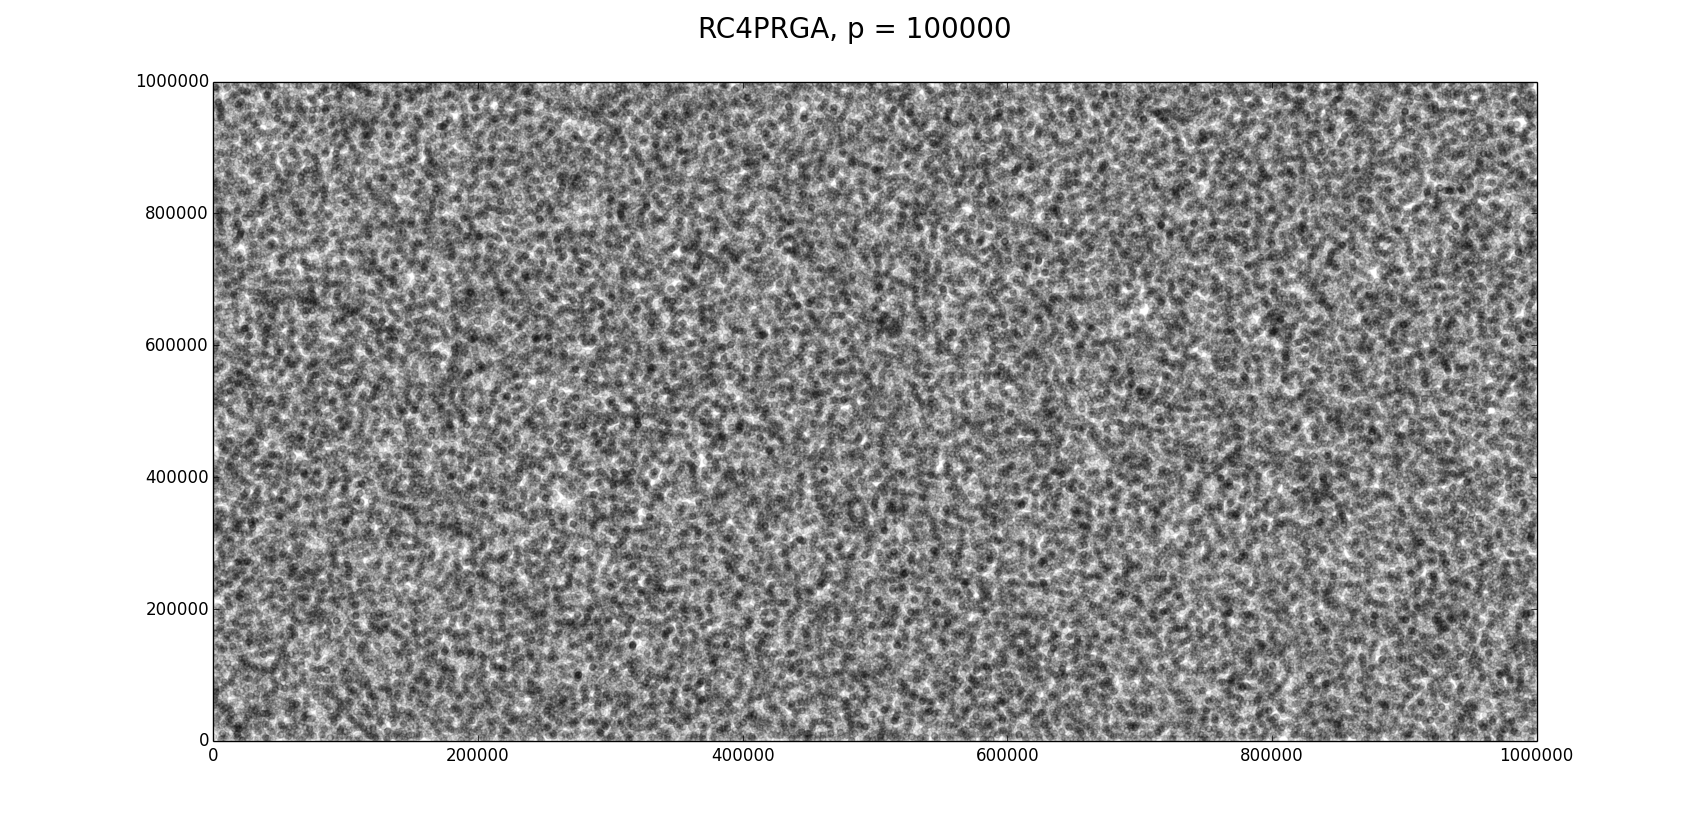
\includegraphics[width=\linewidth]{img/rc4-1.png}

%------------------------------------------------------------------- %
\subsection{Multiply-With-Carry}
Algorytm wymyślony przez George'a Marsaglia. Jego głównymi zaletami jest szybkość i wysoki okres (od ok. $2^{60} $ do $2^{2000000}$).
MWC opiera sie na operacji modulo liczby b (zazwyczaj wynosi ona $2^{32}$ dlatego, że w większości komputerów standardowa operacja) 
Generator wymaga podstawy $b$ mnożnika $a$ , zbioru $x$ losowych wartości takich że r zawiera sie w $b$ i początkowego przeniesienia $c < a$. 
Algorytm wygląda następująco:
$$(1)\ t:=a \times x + c $$
$$(2)\ x:= t \bmod  b $$
$$(3)\ c:= (int)\ t/b$$
Warto zauważyć, że przy arytmetyce $b=2^{32}$ wartość $c$ będzie generowana przez pierwsze 32 bity liczby, natomiast kolejna wartość x przez dolne 32 bity. Mnożnik $a$ jest dobrany w taki sposób aby $ab-1$ i $(ab-1)/2$ były liczbami pierwszymi.
\newline Generator MWC przechodzi testy statystyczne, których generatory LCG nie przechodzą. Przez ten fakt MWC rozważany był jako algorytm kryptograficznie bezpieczny. Jednak badania pokazują, że bity generowane są lekko stronniczo, co przekreśla go w zastosowaniach kryptograficznych. Zostało to naprawione w generatorze CMWC (Complimentary Multiply with Carry).\\
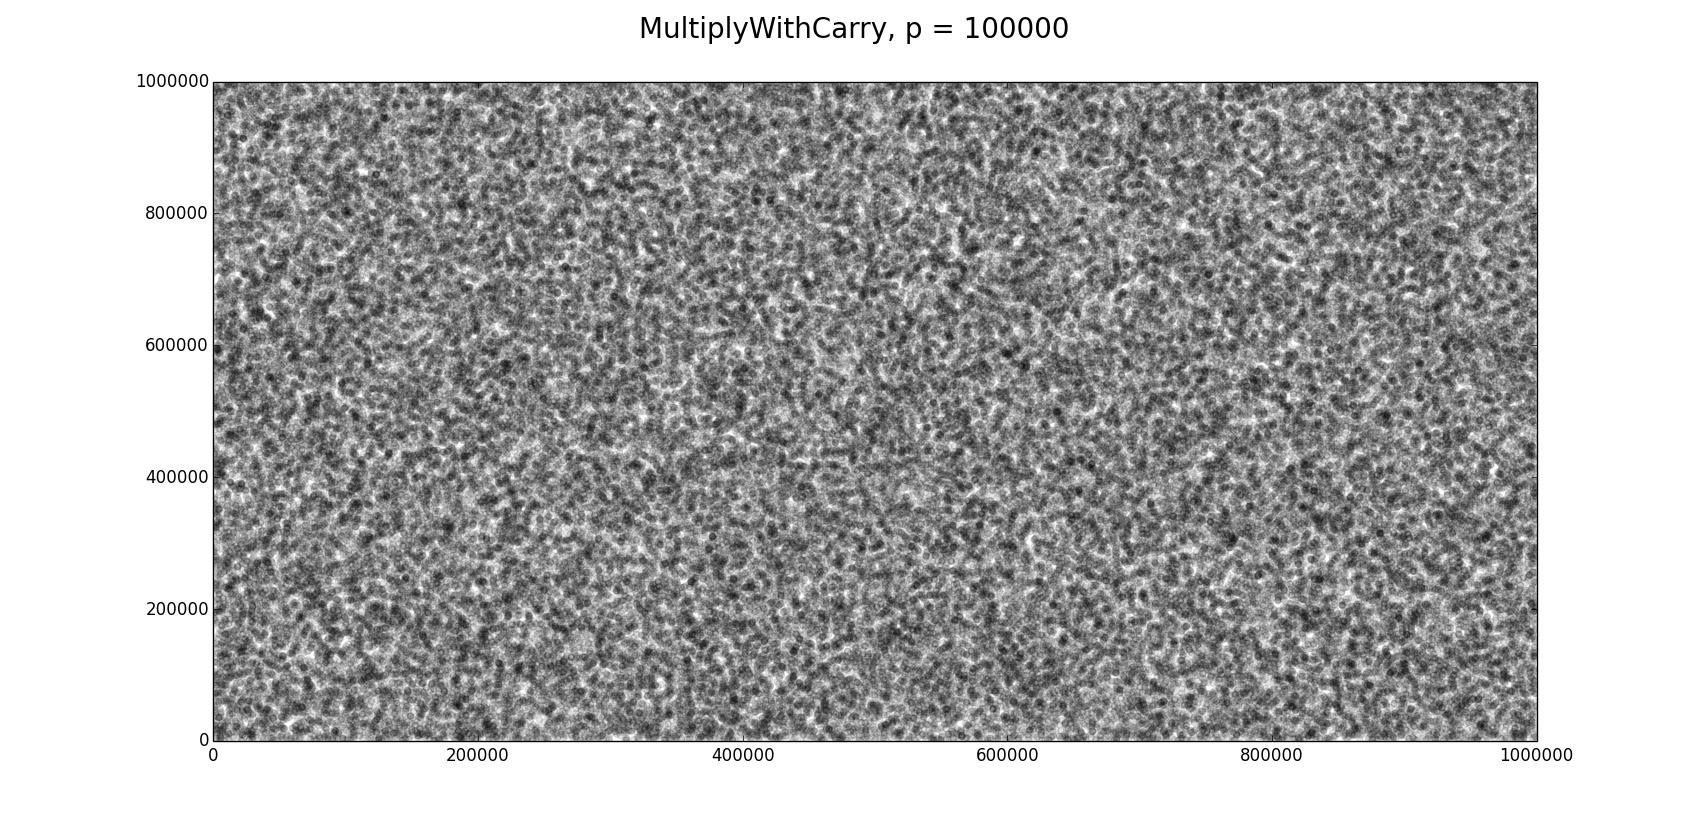
\includegraphics[width=\linewidth]{img/mwc-1.png}

%------------------------------------------------------------------------------------------------ %
	

    \subsection{Lagged-Fibonacci-Generator}
    Generator Fibonacciego jest jednym z wielu wariantów uogólnionego generatora liniowego liczb losowych. \\
    Generator korzysta z ciągu Fibonacciego, stąd wzór:
    $X_{n}=X_{n-1}+X_{n-2}$ \textit{mod m}
    Generator Fibonacciego ma dużo lepsze parametry jakościowe od innych generatorów liniowych, ale wymaga dużo większego nakładu obliczeń przy generacji, co wiąże się z czasem. Wadą tego generatora są duże korelacje między wyrazami ciągu. Ciągi te spełniają warunek rozkładu, ale nie spełniają warunku niezależności.


%----------------------------------------------------------------------------------------

%\section*{Wnioski}


%----------------------------------------------------------------------------------------
%	BIBLIOGRAPHY
%----------------------------------------------------------------------------------------

%\bibliographystyle{unsrt}

%\bibliography{sample}

%----------------------------------------------------------------------------------------

\end{document}